% Editable architecture diagram. Compile with XeLaTeX from this directory.
% Fonts: Plus Jakarta Sans, distributed with OFL in fonts/.
\documentclass[tikz,border=0pt]{standalone}
\usepackage{fontspec}
\hyphenpenalty=10000
\usepackage{tikz}
\usetikzlibrary{arrows.meta,calc,shadings}
\setmainfont[Path=fonts/,Extension=.ttf,UprightFont=*-Regular,BoldFont=*-Bold]{PlusJakartaSans}
\definecolor{navy}{HTML}{061723}
\definecolor{navyblue}{HTML}{10233F}
\definecolor{surface}{HTML}{102C40}
\definecolor{edge}{HTML}{28566B}
\definecolor{cyan}{HTML}{00E5FF}
\definecolor{turquoise}{HTML}{00B4D8}
\definecolor{sky}{HTML}{4CC9F0}
\definecolor{whiteink}{HTML}{EEF7FC}
\definecolor{muted}{HTML}{A4BDCC}
\definecolor{deep}{HTML}{0B2233}
\newcommand{\textat}[6]{\node[anchor=north west,inner sep=0pt,text width=#3cm,align=left,text=#5,font=\fontsize{#4}{\numexpr#4+4\relax}\selectfont] at (#1,#2) {#6};}
\newcommand{\card}[6]{%
  \node[draw=#5,line width=0.65pt,fill=surface,rounded corners=5pt,minimum width=5.1cm,minimum height=2.65cm,inner sep=0pt] (#1) at (#2,#3) {};
  \textat{#2-2.28}{#3+1.02}{4.56}{13}{whiteink}{\textbf{#4}}
  \textat{#2-2.28}{#3+0.20}{4.56}{9}{muted}{#6}
}
\begin{document}
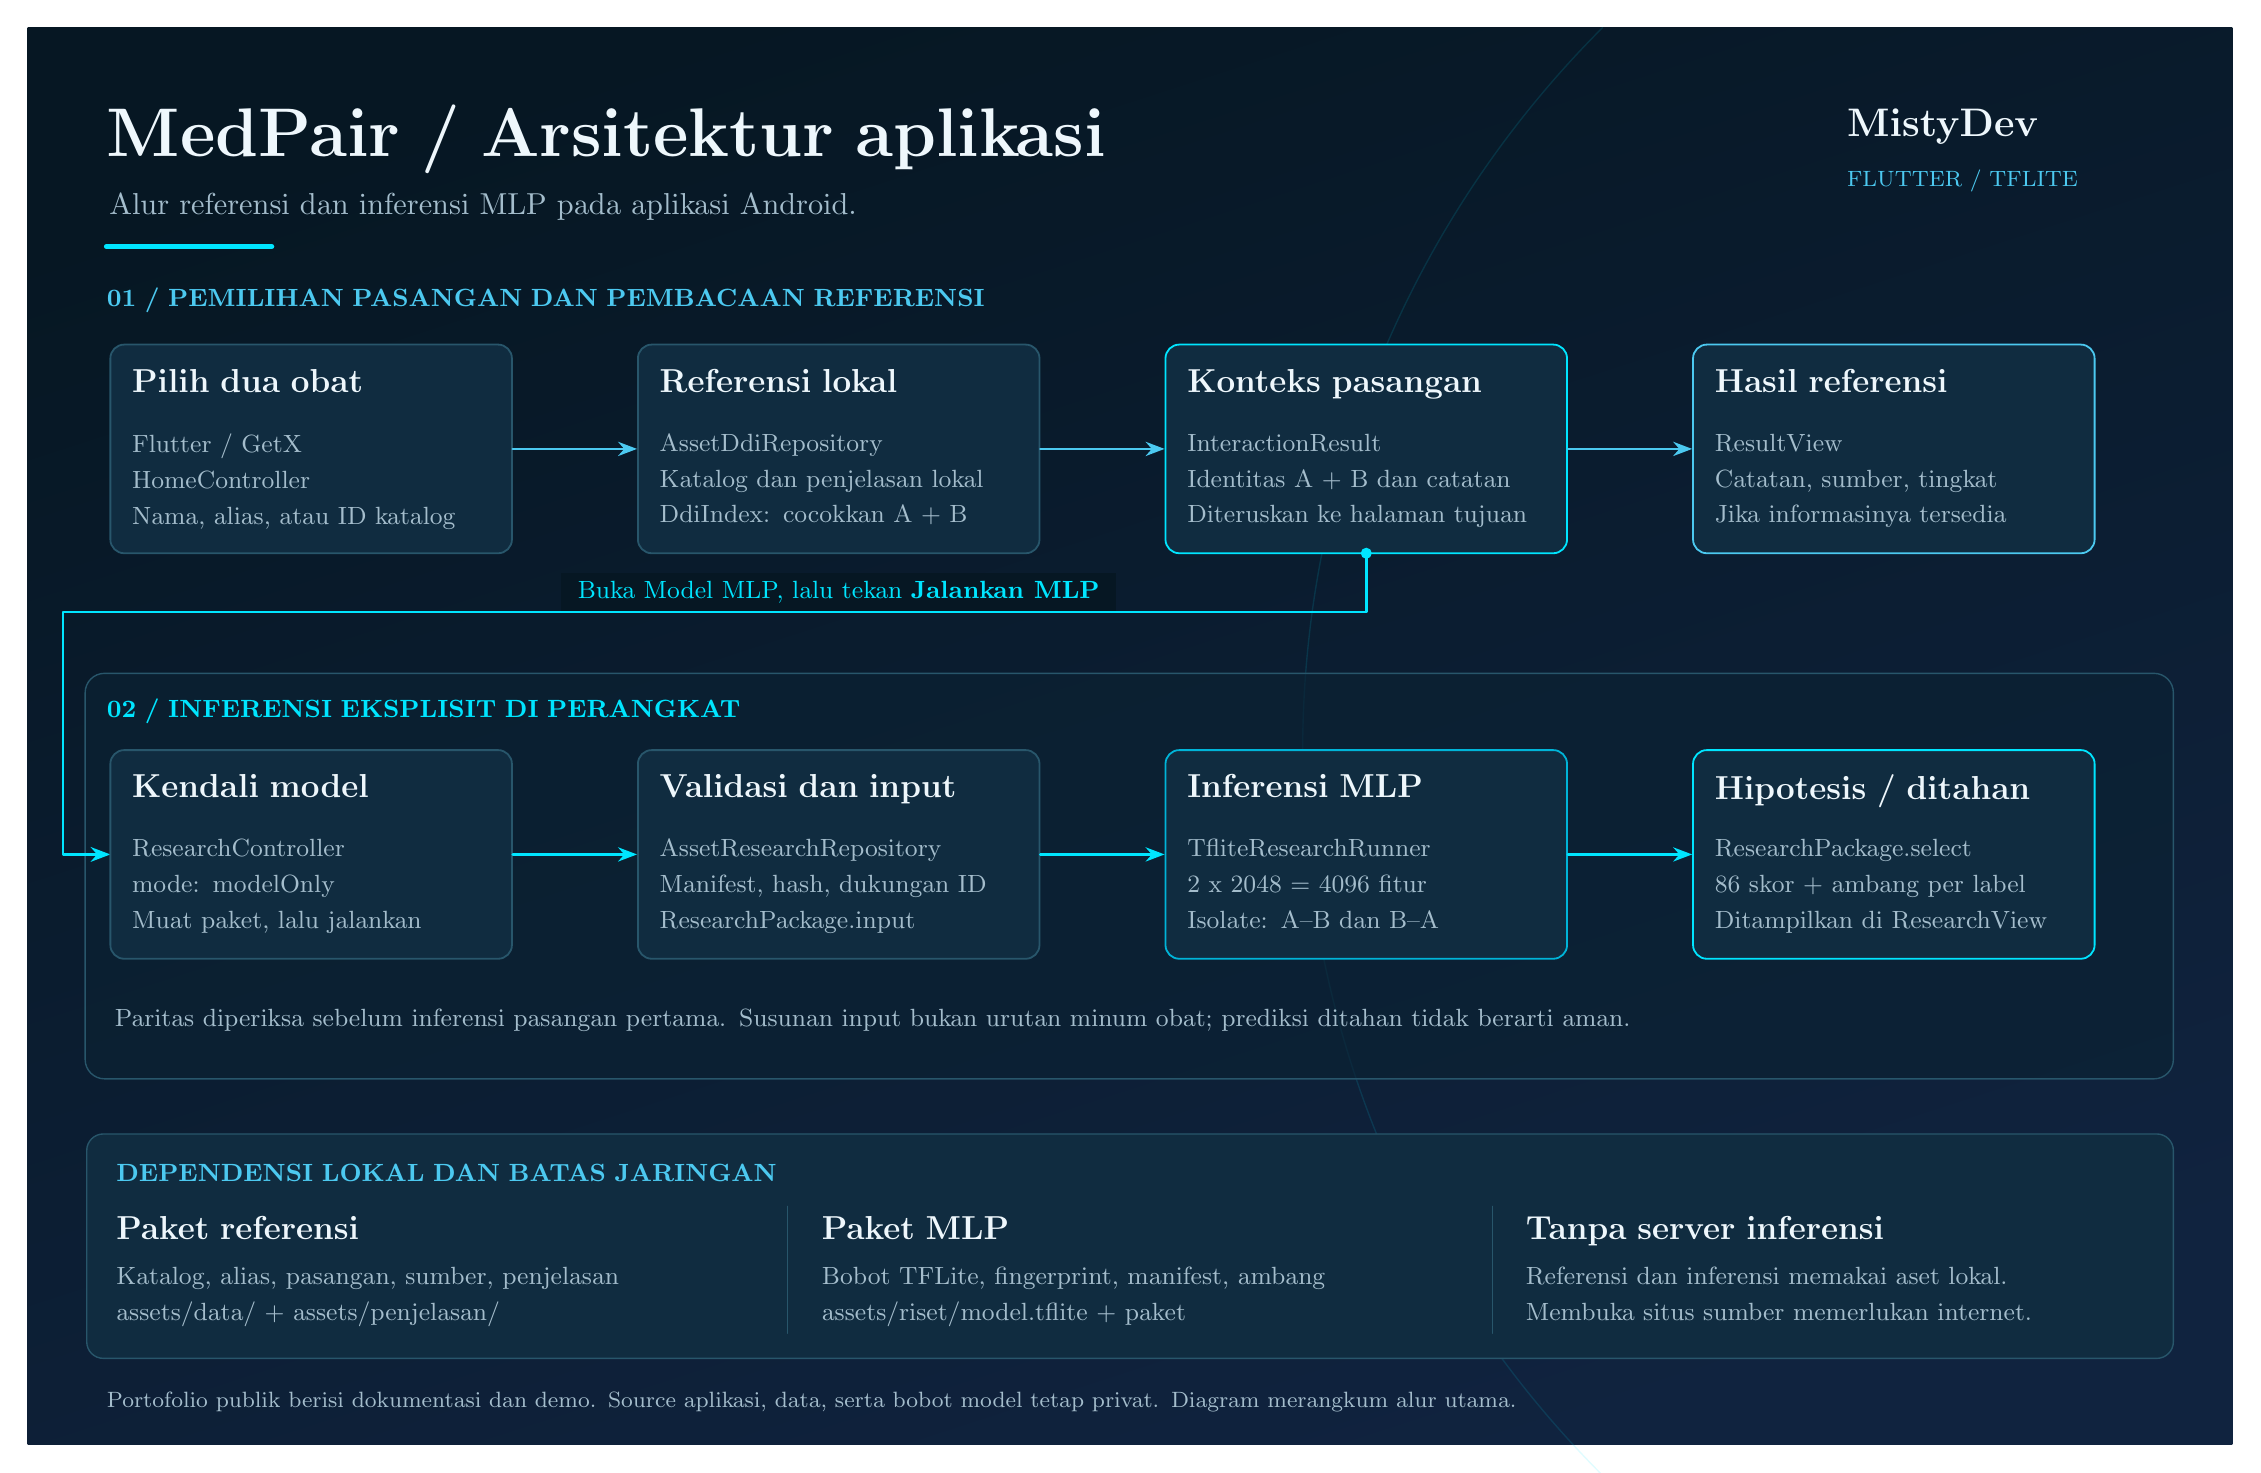
\begin{tikzpicture}[x=1cm,y=1cm,>=Stealth,line cap=round,line join=round]
  \path[use as bounding box] (0,0) rectangle (28,18);
  \shade[left color=navy,right color=navyblue,shading angle=18] (0,0) rectangle (28,18);
  \draw[cyan,opacity=.12,line width=.5pt] (20,18) arc[start angle=135,end angle=225,radius=13cm];
  \textat{1.0}{17.03}{19}{25}{whiteink}{\textbf{MedPair / Arsitektur aplikasi}}
  \textat{1.03}{15.90}{21}{11}{muted}{Alur referensi dan inferensi MLP pada aplikasi Android.}
  \textat{23.1}{16.98}{3.8}{15}{whiteink}{\textbf{MistyDev}}
  \textat{23.1}{16.20}{3.8}{8}{sky}{FLUTTER / TFLITE}
  \draw[cyan,line width=1.8pt] (1.0,15.22)--(3.1,15.22);
  \textat{1.0}{14.70}{23}{9}{sky}{\textbf{01 / PEMILIHAN PASANGAN DAN PEMBACAAN REFERENSI}}

  \card{ui}{3.6}{12.65}{Pilih dua obat}{edge}{Flutter / GetX\par HomeController\par Nama, alias, atau ID katalog}
  \card{ref}{10.3}{12.65}{Referensi lokal}{edge}{AssetDdiRepository\par Katalog dan penjelasan lokal\par DdiIndex: cocokkan A + B}
  \card{pair}{17.0}{12.65}{Konteks pasangan}{cyan}{InteractionResult\par Identitas A + B dan catatan\par Diteruskan ke halaman tujuan}
  \card{result}{23.7}{12.65}{Hasil referensi}{sky}{ResultView\par Catatan, sumber, tingkat\par Jika informasinya tersedia}
  \foreach \a/\b in {ui/ref,ref/pair,pair/result}{\draw[-{Stealth[length=2.4mm]},sky,line width=1.0pt] (\a.east)--(\b.west);}

  \path[draw=edge,fill=deep,fill opacity=.65,rounded corners=7pt,line width=.5pt] (.73,4.65) rectangle (27.25,9.8);
  % The model route receives InteractionResult; reference data is not bypassed.
  \draw[cyan,line width=1.0pt,-{Stealth[length=2.5mm]}] (pair.south)--(17,10.58)--(.45,10.58)--(.45,7.5)--(1.05,7.5);
  \fill[cyan] (17,11.325) circle[radius=2pt];
  \node[anchor=south,fill=navy,inner xsep=6pt,inner ysep=3pt,text=cyan,font=\fontsize{9}{12}\selectfont] at (10.3,10.58) {Buka Model MLP, lalu tekan \textbf{Jalankan MLP}};

  \textat{1.0}{9.48}{24}{9}{cyan}{\textbf{02 / INFERENSI EKSPLISIT DI PERANGKAT}}
  \card{controller}{3.6}{7.5}{Kendali model}{edge}{ResearchController\par mode: modelOnly\par Muat paket, lalu jalankan}
  \card{package}{10.3}{7.5}{Validasi dan input}{edge}{AssetResearchRepository\par Manifest, hash, dukungan ID\par ResearchPackage.input}
  \card{runner}{17.0}{7.5}{Inferensi MLP}{turquoise}{TfliteResearchRunner\par 2 x 2048 = 4096 fitur\par Isolate: A--B dan B--A}
  \card{output}{23.7}{7.5}{Hipotesis / ditahan}{cyan}{ResearchPackage.select\par 86 skor + ambang per label\par Ditampilkan di ResearchView}
  \foreach \a/\b in {controller/package,package/runner,runner/output}{\draw[-{Stealth[length=2.4mm]},cyan,line width=1.0pt] (\a.east)--(\b.west);}
  \textat{1.10}{5.54}{25.5}{9}{muted}{Paritas diperiksa sebelum inferensi pasangan pertama. Susunan input bukan urutan minum obat; prediksi ditahan tidak berarti aman.}

  \path[draw=edge,fill=surface,rounded corners=6pt,line width=.5pt] (.75,1.10) rectangle (27.25,3.95);
  \textat{1.12}{3.57}{24}{9}{sky}{\textbf{DEPENDENSI LOKAL DAN BATAS JARINGAN}}
  \draw[edge,line width=.5pt] (9.65,1.42)--(9.65,3.03);
  \draw[edge,line width=.5pt] (18.60,1.42)--(18.60,3.03);
  \textat{1.12}{2.91}{8.0}{12}{whiteink}{\textbf{Paket referensi}}
  \textat{1.12}{2.26}{8.0}{9}{muted}{Katalog, alias, pasangan, sumber, penjelasan\par assets/data/ + assets/penjelasan/}
  \textat{10.08}{2.91}{8.1}{12}{whiteink}{\textbf{Paket MLP}}
  \textat{10.08}{2.26}{8.1}{9}{muted}{Bobot TFLite, fingerprint, manifest, ambang\par assets/riset/model.tflite + paket}
  \textat{19.02}{2.91}{7.7}{12}{whiteink}{\textbf{Tanpa server inferensi}}
  \textat{19.02}{2.26}{7.7}{9}{muted}{Referensi dan inferensi memakai aset lokal.\par Membuka situs sumber memerlukan internet.}
  \textat{1.0}{.68}{26}{8}{muted}{Portofolio publik berisi dokumentasi dan demo. Source aplikasi, data, serta bobot model tetap privat. Diagram merangkum alur utama.}
\end{tikzpicture}
\end{document}
